\documentclass[11pt]{article}
\usepackage{acl2014}
\usepackage{times}
\usepackage{url}
\usepackage{latexsym}
\usepackage{graphicx}

% Change this if needed to set titlebox size.
%\setlength\titlebox{5cm}

\title{LING 573: Initial Project Report}

\author{Clara Gordon \\
  University of Washington \\
  Seattle, WA \\
  {\tt cgordon1@uw.edu} \\\And
  Claire Jaja \\
  University of Washington \\
  Seattle, WA \\
  {\tt cjaja@uw.edu} \\\And
  Andrea Kahn \\
  University of Washington \\
  Seattle, WA \\
  {\tt andrea.m.kahn@gmail.com} \\}

\date{}

\begin{document}
\maketitle
\begin{abstract}

We implemented a question answering system to handle factoid questions from the QA track of the Text Retrieval Conference (TREC), using the AQUAINT Corpus of English News Text as a document collection.

\end{abstract}

\section{Introduction}

Question answering (QA) has long been a prominent problem in the field of natural language processing. In contrast to information retrieval (IR) systems, which return relevant documents based on search terms, a question answering system takes a natural-language question as input and outputs a natural-language answer. IR is typically a component of the system, but the addition of question and answer processing prevents users from having to sift through long documents to find the information they are seeking.

We implemented a question answering system to handle factoid questions from the QA track of the Text Retrieval Conference (TREC), using the AQUAINT Corpus of English News Text as a document collection.

\section{System Overview}

Our system is coded in Python. Third-party modules that we use include Indri/Lemur (for IR), Pymur (a Python wrapper for Indri/Lemur), Beautiful Soup (for XML parsing), NLTK (for tokenization). We chose Indri/Lemur for IR because of its specific handling of TREC-formatted question files. We currently use a stopword list taken from the Indri/Lemur documentation.

\begin{figure}
  \centering
    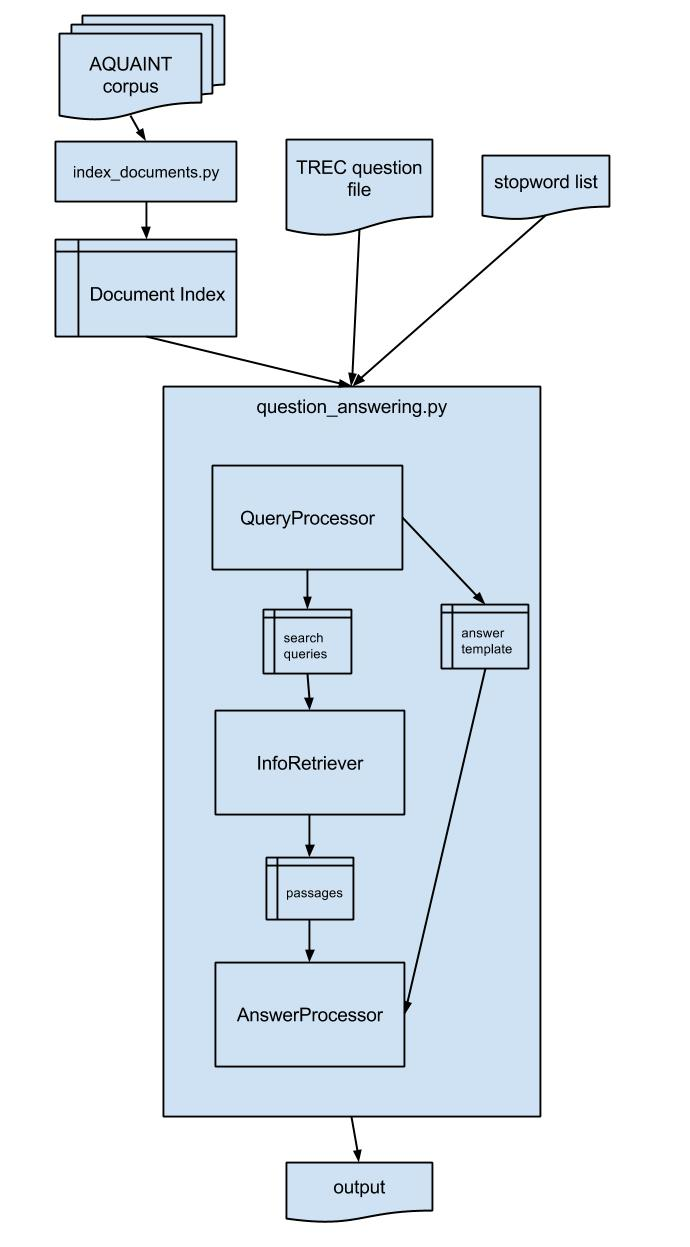
\includegraphics[width=0.5\textwidth]{system_architecture.jpg}
 \caption{System architecture.}
\end{figure}

\section{Approach}

The question answering system is run by a wrapper script, question\_answering.py, which takes as arguments a file containing questions in TREC QA format, a path to the document index, a run tag, and a path to the desired output file. It uses the third-party module Beautiful Soup to parse the XML in the TREC document and generate a list of questions. It then passes the questions one-by-one to the pipeline described below. For each question, for each answer returned, it prints the question, the run tag, the document ID associated with the answer, and the answer to the output file.

Classes that are used by multiple modules in the pipeline are defined in the module general\_classes.py. These include:

\begin{itemize}
\item Question class: A Question object stores as attributes the TREC question ID, the question type, the TREC natural-language question stored as a string, and the "target" (the context given for a set of questions in TREC 2004-2006; defaults to None).
\item SearchQuery class: A SearchQuery object stores as attributes a dictionary of search terms, each of which can be one or more words, mapped to weights indicating how important those terms are perceived as being, and an overall weight for the query, which will be used to calculate the probability of the corresponding AnswerCandidate.
\item AnswerTemplate class: An AnswerTemplate object stores as attributes a set of basic search query terms from the original question and a dictionary for the weights of each NE type, where the weights will be used to reweight AnswerCandidate objects during answer processing.
\item Passage class: A Passage object stores as attributes the text of a passage returned by Indri/Lemur, a weight, and the ID of the document from which this passage was extracted.
\end{itemize}

\subsection{System architecture}

Our pipeline for the processing of a single question consists of three components, described below. The pipeline takes a Question object as input and outputs a list of AnswerCandidate objects.

\subsubsection{Query processing}

The query processing module is responsible for creating one or more weighted search queries (which are passed to the information retrieval module to be used for passage retrieval) and instantiating an answer template (which is passed to the answer processing module to be used during answer ranking). A QueryProcessor object is instantiated with a Question object and generates a vocabulary, a list of words (i.e., whitespace-tokenized strings) occurring in the question/target and their counts. This vocabulary is used to instantiate an AnswerTemplate object. (In subsequent versions of the system, we plan to implement a more sophisticated approach toward answer template creation, including question classification.)

The QueryProcessor is then used to generate a list of weighted search queries, each of which is in turn a set of weighted search terms. In the current version of the system, the QueryProcessor generates just one search query, which is the set of words occurring in the question and target with their counts as weights. In subsequent versions of the system, we plan to explore more sophisticated methods of query generation, including query expansion, as well as to test generating multiple weighted search queries for one question.

\subsubsection{Information retrieval}

The infomation retrieval module uses the Indri/Lemur IR system to retrieve a series of twenty snippets and associated documents for each set of query terms passed to it by the query processing module. Although the Python wrapper pymur is used to index the document collection, this portion of the system uses the subprocess module to directly query Indri using command line arguments. This is necessary because certain Indri functions, such as snippet retrieval, are not available in the wrapper. 

Once the snippets and associated document metadata are retrieved from standard out, a series of character-based split commands is used to segment the string into the relevant fields: document ID number, document weight, and snippet text. These fields are used to construct a Passage object. A list of these objects is then passed to the answer processing module, which uses the snippets and associated metadata to derive answer candidates.   

\subsubsection{Answer candidate extraction and ranking}

In order to extract and rank answers, the AnswerProcessor class is used.  An object of this class is initialized with a list of Passage objects, an AnswerTemplate object, and an optional stopword list.  This object can then generate and rank answers.  This is done in a series of steps.

First, possible answers are extracted from the Passages by generating all unigrams, bigrams, trigrams, and 4-grams from the text of each passage; the score of each of these possible answers is the sum of the negated inverse of the retrieval score of the passages it is found in.  If an n-gram appears multiple times in a passage, the n-gram's score is updated each time the n-gram appears, so a possible answer that appears frequently in a passage is scored higher than one that appears just once in the passage.  The negated inverse of the retrieval score is used because Indri/Lemur returns a negative score where higher (i.e. closer to zero) is better; we wanted a positive score where higher (i.e. further from zero) is better for our own readability for troubleshooting.  While these scores are being calculated, the document IDs where the n-grams occur are also being tracked for later use.  At the end, a list of AnswerCandidate objects is generated which contains a possible answer, its score, and the documents it is found in.

After this, the AnswerCandidates go through a filtering step.  At this step, any answers that start or end with a stopword or contain any words from the original query (retrieved from the AnswerTemplate) or any standalone punctuation tokens are discarded.  Then, a combining step updates the score of each answer to be the current score plus the sum of the scores of the unigram answers contained within it; this prevents unigrams from being the highest ranked answers and instead favors longer answers.

Next, the answers are reweighted.  At this point, any answers that did not appear in more than one passage are discarded.  Additionally, this is the place where constraints on named entity type from the AnswerTemplate can be applied to increase or decrease AnswerCandidate scores; currently, since no constraints are being generated at the query processing stage, there is nothing to apply.

Lastly, the answers are ranked by score, and the top 20 are returned.  When the output is generated, for each answer, one of the document IDs where it occurred is randomly selected as the source of the answer.  In future development, a more clever method for selecting which document ID to use as the answer source will be employed.

\section{Results}

We evaluated our results using the mean reciprocal rank (MRR) measure with strict and lenient evaluation. At this point, we are reporting only baseline results, shown in Table 1 below.

\vspace{5mm}
{\centering
\begin{tabular}{|c|c|c|}
\hline
\textbf{System} & \textbf{Strict} & \textbf{Lenient} \\ \hline
Baseline & 0.00511 & 0.02894 \\ \hline
\end{tabular}

\vspace{1mm}
\emph{Table 1: Baseline results based on automatic pattern scoring. All scores rounded to five significant digits.}
\par}

\section{Discussion}

Our baseline results are very low.  Error analysis indicates that this is most likely the result of the low quality of the snippets returned at retrieval time.  Additionally, there are some duplicate documents, so an answer may be retained as being from more than one document when in reality, it is from two identical documents and should be treated as being from one document and thus discarded.

In subsequent versions of the system, we hope to address the first issue by augmenting the query processing module to include query expansion. Better search queries (and more of them) will hopefully improve the quality of the snippets returned in the information retrieval module.

In addition, we plan to encode more information in the answer template by implementing question classification in the query processing module. This will hopefully facilitate better answer generation and ranking in the answer processing module.

\section{Conclusion}

\nocite{*}
\bibliographystyle{acl}
\bibliography{D2references}

%\begin{thebibliography}{}

%\end{thebibliography}

\end{document}
